\section{Clustering}


\subsection{Clustering with Gaussian Mixture Model}
One way to cluster data is with a Gaussian Mixture Model (GMM). This model uses a
probabilistic estimation of densities trained, in this report, with the
Expectation Maximizaion (EM) algorithm.\\
The GMM uses multivariate normal distributions as the distribution, which means
each cluster has assigned a mean ($\mu$) and a covariance matrix ($\Sigma$) to it.
This means that a given observation, depending on these two parameters and the
observation itself, has a probability of belonging to each cluster. Then, the
cluster witch the observation is most likely to belong to is the cluster the
observation is assigned to.\\
The first thing to do is find out the amount of clusters the GMM should aim for.
This is done with cross-validation (where the negative log-likehood should be
as low as possibe), Akaike's information Criterion (AIC) and Bayesian Information
Criterion (BIC). AIC and BIC should be low as well, so Figure \ref{cv}, showing
cross-validation, AIC and BIC for different amount of clusters, is helpful when
determining number of clusters.\\
\begin{figure}[htbp]
  \centering
  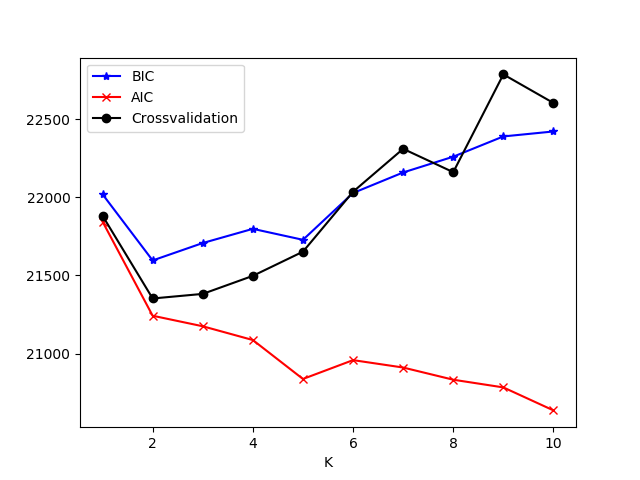
\includegraphics[width=\textwidth]{Figure_1.png}
  \caption{BIC, AIC and crossvalidation for different numbers of clusters}
  \label{cv}
\end{figure}
The BIC and negative log-likelihood are both low at k=2, while AIC continues
decreasing up to k=10. The BIC and AIC penalize model complexity in different ways,
and it is often the case that AIC prefers the more complex model. With this in mind,
k=2 is used for the modelling in this section. It could be argued with reference to AIC
that the number of clusters should be higher, but this take will not be considered here.\\
The 2 clusters projected down on the 2 attributes explaining the higest amount
of variance (insulin and glucose, responsible for more than 95\% of the total
variance) can be seen in Figure \ref{gmm}.\\
\begin{figure}[htbp]
  \centering
  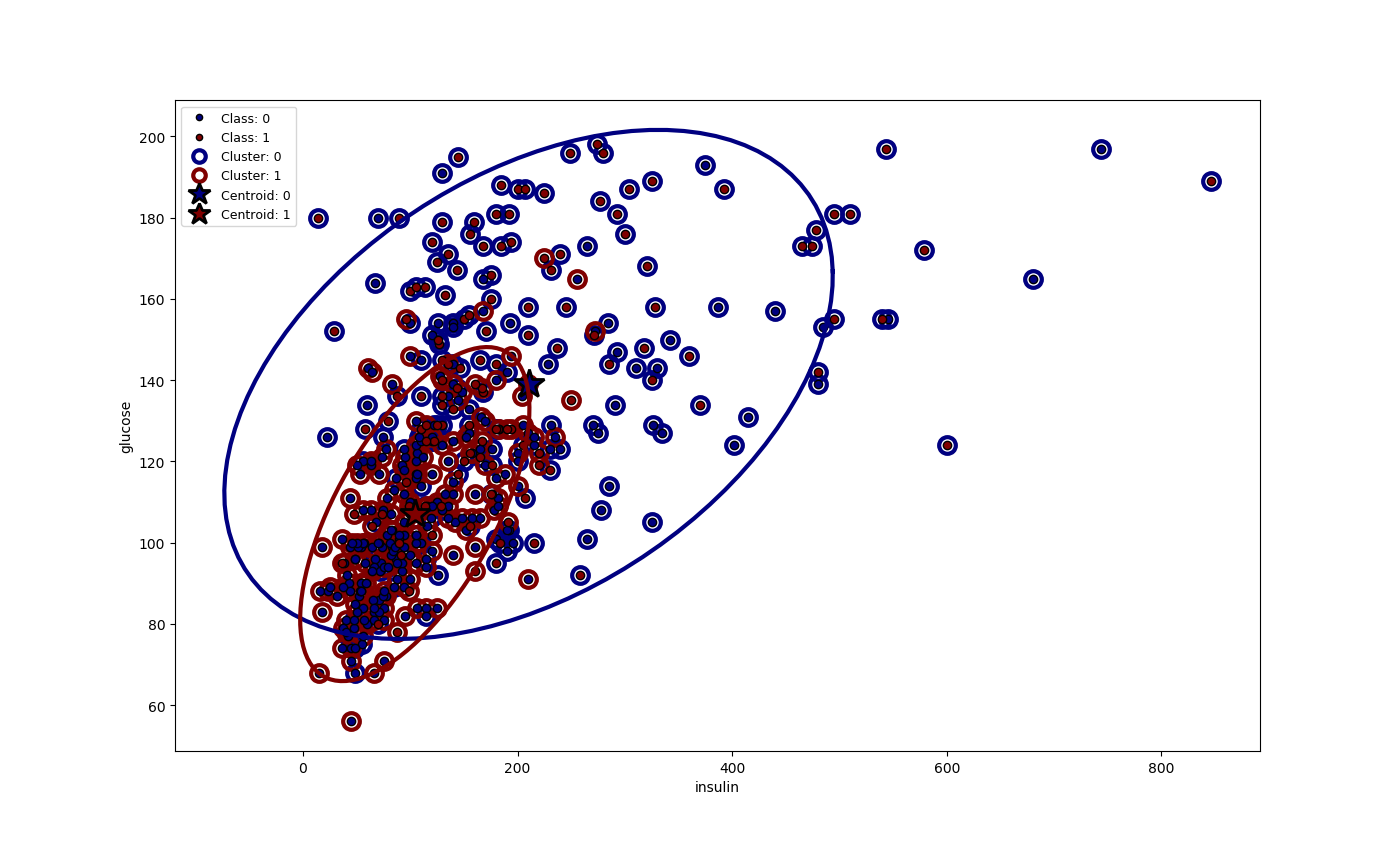
\includegraphics[width=\textwidth]{Figure_2.png}
  \caption{GMM clustering in 2 dimensions}
  \label{gmm}
\end{figure}
Qualitatively inspecting the data shows cluster 1 (red circles), which one
will most likely belong when having both low glucose and insulin (centered
at the bottom left red star). Also, cluster 1 seems, in this plane, to be more
an ellipsoid than a circle. Cluster 0 is more spread out and more circular, with
an ellipsoid than a circle. Cluster 2 is more spread out and more circular, with
center at higher glucose and insulin levels.
Because only 2 attributes are presented in the plot, not all the variance is
explained, which is why the clustering seems a bit inconsistent in 2 dimensions.
Plotting against the first and second principal components could show the clusters better
in 2 dimensions but might be harder to interpret. In the 8-dimensional space, the centers
of the clusters have the coordinates presented in Table \ref{cent}. \\
This table shows that the centers of the two clusters also are placed very differently
in the age direction and in the pregnancies direction, where both values are
higher for the centre of cluster 0.\\
\begin{table}[h]
\centering
\begin{tabular}{ccccccccc}
    & pregnancies & glucose & bp & thickness & insulin & bmi & diapedig & age\\
$\mu$_0 & 4.96 & 138.95 & 74.51 & 31.36 & 210.28 & 34.59 & 0.61 & 37.56 \\
$\mu$_1 & 1.71 & 107.04 & 66.99 & 27.03 & 104.26 & 31.65 & 0.44 & 24.57 \\
\end{tabular}
\caption{Centroids coordinates}
\label{cent}
\end{table}

\subsection{Hierarchical clustering}
Hierarchical clustering is a deterministic way of clustering observations. The
point is start off by assigning each observation to its own cluster and then
merge clusters that are closest to each other. Before initializing the algorithm,
it is neccessary to specify how the distance between clusters is defined. In this
report, the distance is defined by Ward's linkage function (which minimizes
the sum-of-squares between each point and the centre of its assigned cluster).
Other linkage functions were considered, but did not perform as well as Ward.
The hierarchical clustering of the data, this time standardized, can be seen
in Figure \ref{dendrogram} represented by a dendrogram with 6 levels.\\
\begin{figure}[htbp]
  \centering
  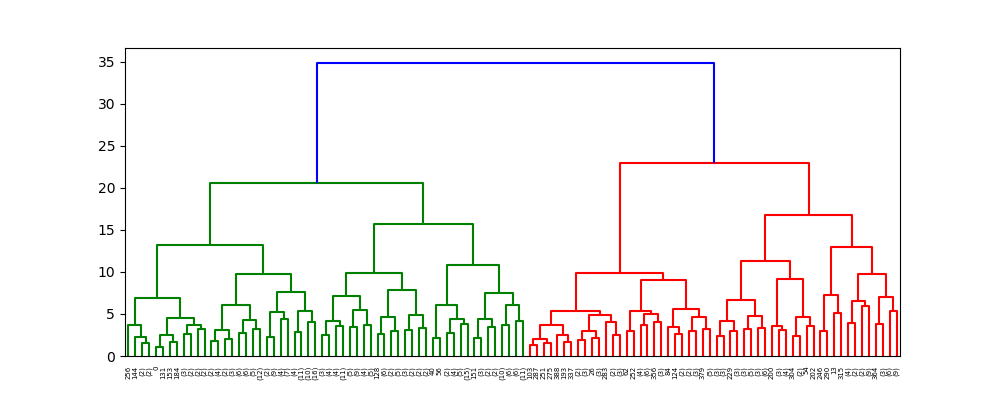
\includegraphics[width=\textwidth]{Figure_3.png}
  \caption{Merging of clusters illustrated with a dendrogram}
  \label{dendrogram}
\end{figure}
Outliers can usually be found by visual inspection of a dendrogram, where the
outliers will join other clusters late. This is, however, difficult to see in
this dendrogram, as the bottom is not visible. In general, the dendrogram seems
quite symmetrical which is a good sign, and the longest vertical lines suggests
2 clusters best describes the data. Plotted against the glucose and insulin attributes,
the scatter-plot in Figure \ref{hc} emerges.\\
\begin{figure}[htbp]
  \centering
  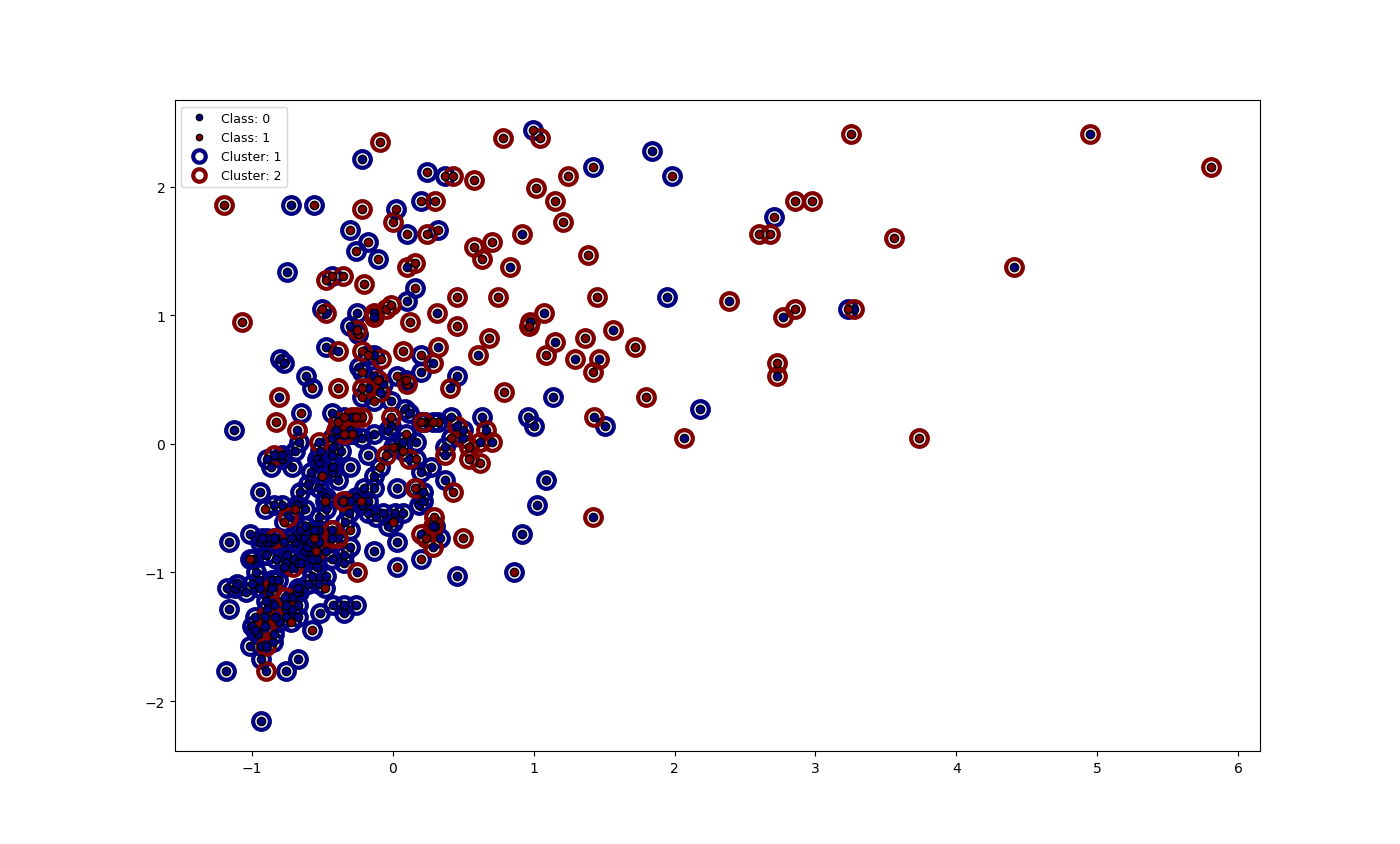
\includegraphics[width=\textwidth]{Figure_4.png}
  \caption{HC in 2 dimensions}
  \label{hc}
\end{figure}
Qualitatively, some of the same structures can be seen as in the scatter plot
of the GMM. Again, some of the observations assigned to, say, cluster 0
surrounded by cluster 1's must somehow be different in a direction not show
on the scatter-plot.

\subsection{Quality of clustering}
In this section, the clusters' validity will be evaluated based on Rand statistic,
Jaccard coefficient and Normalized Mutual Information (NMI). The hierarchical clustering,
using Ward linkage, will be cut off making 2 clusters (which, based on where the
longest vertical lines are in the dendrogram, seems reasonable) and then
compared to the GMM. Both models produce two clusters. These clusters' similarity
with the "clustering" of the label of the data (here, the binary attribute telling
whether a patient is sick or nor) will be used to determine the quality of validity
of the GMM and hierarchical clustering.\\
 Table \ref{clusteval} gives an overview of the performances:\\
\begin{table}[h]
\centering
\begin{tabular}{ccccc}
    & Rand & Jaccard & NMI\\
GMM & 0.59 & 0.44 & 0.15 \\
HC & 0.58 & 0.45 & 0.09 \\
\end{tabular}
\caption{Clustering evaluation scores}
\label{clusteval}
\end{table}

The Rand score or the Rand index is defined as the sum of object pairs with
the same label assigned to the same cluster and object pairs with different
labels assigned to different clusters divided by the total number of pairs. The
Jaccard score or the Jaccard index is similar, however, the number of object
pairs with different labels assigned to different clusters are subtracted from
the denominator rather than added to the numerator, assigning (usually) less
importance to observations scattered in many clusters. Judging from Rand and
Jaccard, the two models cluster equally well.\\
NMI is quite low for both kinds of clustering. This number tells something about
how informative to partitions are about each other and should be 1 if the clustering
catches the labels spot on. This number is a bit higer for the GMM than for the hierarchical
clustering, but is still low enough to not place too much confidence in trusting either
of these two models to represent the labels with their clustering.

\section{Outlier detection}
\begin{figure}[htbp]
  \centering
  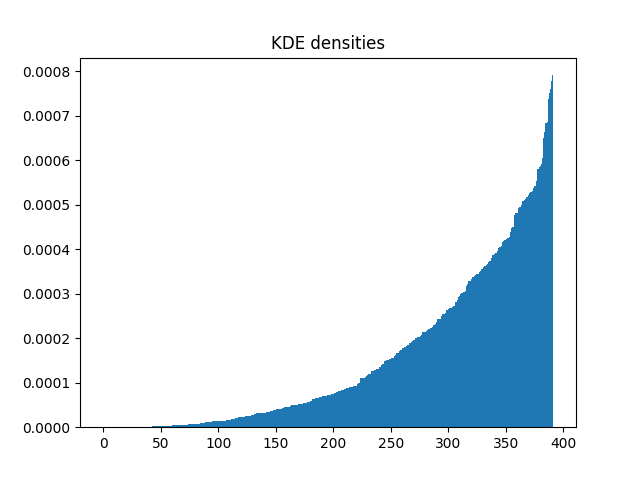
\includegraphics[width=\textwidth]{kde_densities}
  \caption{Density at our data points as estimated by KDE}
  \label{fig:kde}
\end{figure}

The KDE plot, figure \ref{fig:kde},
doesn't tell us much,
the falloff is too smooth
for there to be an obvious cutoff.
As such,
we will be judging outliers based on the
density estimates by KNN,
where there is a sharper falloff at the lower densities.

\begin{figure}[htbp]
  \centering
  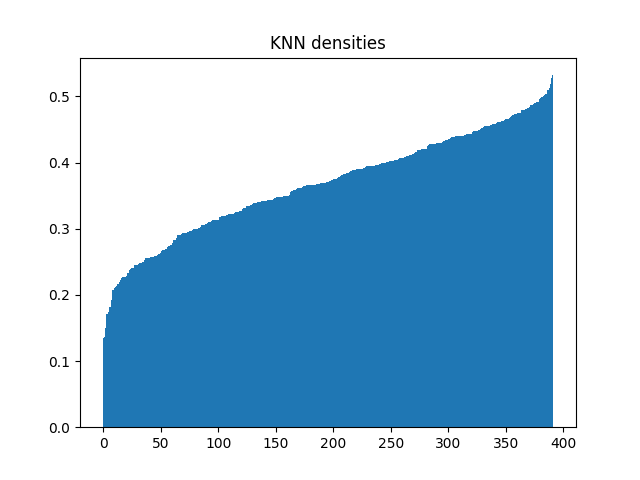
\includegraphics[width=\textwidth]{knn_densities}
  \caption{Density at our data points as estimated by KNN}
  \label{fig:knn}
\end{figure}

The density and average relative density are qualitatively rather similar,
as seen on figures \ref{fig:knn} and \ref{fig:knn-avg-rel}, respectively.
Sorted by density,
most points have only slightly different densities than the points
above and below them.
However, there is a sharp falloff,
with a handful of the points located at the lowest densities
suddenly ``dropping off the density curve''
that the other points seem to follow.
These are the points we consider to be outliers.
For the density, respectively average relative density,
this occurs at $0.2$, respectively $0.6$.
Another point that might be chosen as a cutoff is
the point where the curves seem to momentarily flatten before continuing.
However, this would lead to a far greater number of outliers,
we have chosen the stricter cutoff.

\begin{figure}[htbp]
  \centering
  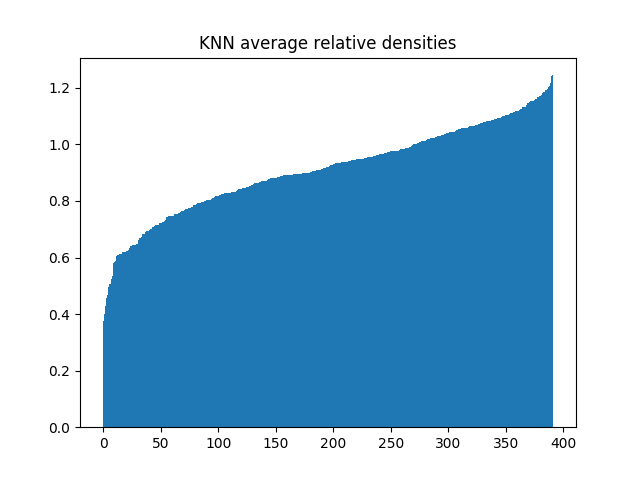
\includegraphics[width=\textwidth]{knn_avg_rel_densities}
  \caption{Average relative density at our data points as estimated by KNN}
  \label{fig:knn-avg-rel}
\end{figure}

As the set of outliers according to the relative density
is a subset of
the set of outliers according to the average relative density,
and because the additional points included seem, intuitively, like outliers
(e.g. the woman who has had 17 pregnancies),
we will be looking at the larger set only.

For a table of the outliers, refer to table \ref{tab:outliers}.

\begin{table}[hbp]
\begin{tabular}{rrrrrrrrr}
pregs & glucose & bp & thickness & insulin & bmi & dia\textunderscore{}pedig & age & class\\
  \hline
0 & 180 & 78 & 63 & 14 & 59.4 & 2.420 & 25 & 1\\
4 & 197 & 70 & 39 & 744 & 36.7 & 2.329 & 31 & 0\\
1 & 189 & 60 & 23 & 846 & 30.1 & 0.398 & 59 & 1\\
0 & 137 & 40 & 35 & 168 & 43.1 & 2.288 & 33 & 1\\
0 & 129 & 110 & 46 & 130 & 67.1 & 0.319 & 26 & 1\\
3 & 173 & 82 & 48 & 465 & 38.4 & 2.137 & 25 & 1\\
0 & 165 & 90 & 33 & 680 & 52.3 & 0.427 & 23 & 0\\
1 & 88 & 30 & 42 & 99 & 55.0 & 0.496 & 26 & 1\\
9 & 134 & 74 & 33 & 60 & 25.9 & 0.460 & 81 & 0\\
17 & 163 & 72 & 41 & 114 & 40.9 & 0.817 & 47 & 1\\
6 & 129 & 90 & 7 & 326 & 19.6 & 0.582 & 60 & 0\\
2 & 197 & 70 & 45 & 543 & 30.5 & 0.158 & 53 & 1\\
\end{tabular}
\caption{Outliers according to average relative density computed by KNN}
\label{tab:outliers}
\end{table}


\section{Association Mining}

\begin{center}
 \begin{tabular}{||c c||}
 \hline
 Attribute number & Attribute \\ [0.5ex]
 \hline\hline
 0 and 9 & Number of times pregnant \\
 \hline
 1 and 10 & Plasma glucose concentration, GTT \\
 \hline
 2 and 11 & Diastolic blood pressure (mm Hg) \\
 \hline
 3 and 12 & Triceps skin fold thickness (mm) \\
 \hline
 4 and 13 & 2-Hour serum insulin ($\mu$ U / ml) \\
 \hline
 5 and 14 & Body mass index Weight in (kg / (Height in $m^2$)) \\
 \hline
 6 and 15 & Diabetes pedigree function \\
 \hline
 7 and 16 & Age (Years) \\
 \hline
 8 and 17 & Class variable, whether or not the person had diabetes (0 or 1) \\ [1ex]
 \hline
\end{tabular}
\end{center}

The association mining gives us an idea of which parameters have an association with each other and if they follow a rule of association.
What is interesting are the parameters which have a high association with each other.
There are two categories that can describe this association:

\textbf{High support:} Which describes if a parameter is rather often involved in the dataset and what are it's probability of getting chosen.

\textbf{High confidence:} Which describes if a parameter is chosen, what other parameter is then most likely to also be chosen, and are there more than one parameter that is likely to get chosen and what are it's/their probability of getting chosen.

When simulating the association mining we set our minSup to 40 and minConf to 80.
It should be noted that not all of our results are listed below due to the support being only 50% or less which we didn't find interesting.

Our results are as follows:
\begin{center}
 \begin{tabular}{||c||}
 \hline
 Frequent itemset number: & Percentage \\ [0.5ex]
 \hline\hline
 17 & Sup. 66.8367 \\
 \hline
 9 & Sup. 54.3367 \\
 \hline
 10 and 17 & Sup. 43.3673 \\
 \hline
 16 and 17 & Sup. 43.3673 \\
 \hline
 13 and 17 & Sup. 42.0918 \\
 \hline
 9 and 17 & Sup. 41.3265 \\
 \hline
 16 and 9 & Sup. 41.3265 \\ [1ex]
 \hline
\end{tabular}
\end{center}

\begin{center}
 \begin{tabular}{||c||}
 \hline
 Association Rule number: & Percentage \\ [0.5ex]
 \hline\hline
 17 <- 10 & Conf. 86.2944, Sup. 43.3673 \\
 \hline
 16 <- 9 and 17 & Conf. 85.8025, Sup. 35.4592 \\
 \hline
 17 <- 16 and 9 & Conf. 85.8025, Sup. 35.4592 \\ [1ex]
 \hline
\end{tabular}
\end{center}

There can clearly be seen pattern here. Parameter 17, or the class variable of having diabetes, clearly has an association with the other parameters.
Which would make the reason for it having so many associations with the other parameters make sense.
There seems to be an association between parameters 16 and 9. Which are the parameters Age and Number of times pregnant. (both, in the upper median)
It would indicate that a female with an age above average also has been pregnant in a number higher than average. Which would make sense.
It seems that parameters 17, 16, 10 and 9 all seem to have an association.
Which we can conclude that if a female has diabetes she seems to also have an age above average, a plasma glucose concentration above average and the number of times pregnant is above average.
This would also make sense biologically.



\appendix
\section{Distribution of responsibilities}

\begin{table}[H]
\centering
\caption{My caption}
\label{my-label}
\begin{tabular}{ll}
\hline
\multicolumn{2}{|l|}{Work distribution} \\ \hline
Part 1              & Andreas                \\
Part 2              & Marcus                 \\
Part 3              & Hildibjørg
\end{tabular}
\end{table}

=======
>>>>>>> 0e01fd7e504c611db29edb1a915bb4271f68a1d8
\subsection{Clustering}

\subsection{Outlier detection/Anomaly detection}

\subsection{Association mining}

\subsection{Previous work}
